\subsection{Data Collection}

In this section the approach and inplementation of data collection for this project is 
examined.

\subsubsection{Requirements for the dataset}

Basic requirements the dataset should fulfill are

\begin{itemize}
    \item \textbf{Includes Spotify song features}

    Spotify provides a set of song features that were generated using their own models.
    The dataset should inlude these features, as they are needed to train the model
    \item \textbf{Includes genre as label}

    The dataset needs to include the genre of the track to use as a label for the classifier
    \item \textbf{Has sufficient sample size per genre}

    In order to train the model well, a sufficient sample size is needed per genre.
    It was not known before collecting the data, how many samples were enough. 
    \item \textbf{Song and Artist name}

    The best way to filter out duplicates is to use the song and artist names.
    Spotify does provide a track id for each song, however, if a song is released twice
    (e.g. as a single and later in an album), these track ids will differ which will lead to a duplicate entry.
\end{itemize}

Additional fields are not going to be used in this analysis, but might still be collected in order to publish the
dataset and enable others to use it for different applications.

\subsubsection{Existing Datasets}

As this paper examines creating a model specifically on Spotify Song Data,
a search on the internet was conducted first, to find a potential pre-made dataset,
pulled from the Spotify \ac{API}, which could be used.
Kaggle \footnote{Kaggle Website: https://www.kaggle.com/} lists an extensive
catalogue of community provided datasets, so the main sources of this search were
Kaggle and Google search for the term "Spotify Song Data".
Kaggle lists a couple of datasets that could be applicable to the research question in
this paper. Some examples of datasets listed are given and explained, why they could not 
be used for this project.

"Spotify music analysis" by user Aeryan \footnote{https://www.kaggle.com/aeryan/spotify-music-analysis}
is a dataset of 2017 rows, which includes musical features like acousticness and tempo,
the song title and artist, but lacks a genre field. Because of the small sample size
and the missing genre field, this dataset could not be used.

There are multiple datasets which include songs that were featured in Spotify's "Top 50" Playlists,
charts, or year in review, recorded at a single point in time or historically.
\footnote{https://www.kaggle.com/nadintamer/top-spotify-tracks-of-2018}
\footnote{https://www.kaggle.com/leonardopena/top50spotify2019}
These could not be used, as the sample size is again too small and the focus is specifically
on the most popular tracks and not a wide variety of music in a genre.

"Dataset of songs in Spotify" \footnote{https://www.kaggle.com/mrmorj/dataset-of-songs-in-spotify}
is the most promising dataset examined, as it has a big sample size and includes genre data.
However, the methodology of how the data was collected is not included and there
could be multiple ways of how genre data for a given song is collected, as is explained later.
Also the genres are limited to very specific directions of Electronic Dance Music and Hip-Hop.

As no optimal dataset for this research paper could be found using our search criteria,
a dataset was specifically created for this paper using the Spotify Web API.

\subsubsection{Ressources and Approach}

Spotify provides extensive documentation for developers on their developer website \footnote {https://developer.spotify.com/}.
This includes development and design guidelines for teams, that want to integrate
Spotify's service into their own apps, documentation on IOS and Android development
a community forum, a developer dashboard and the Web API documentation, which is the main ressource
for data collection from Spotify.

The \ac{API} is based on the \ac{REST} architecture. The different endpoints return JSON metadata
directly from the Spotify Data Catalogue \cite[]{SpotifyWebAPI}. There are also features to query for
user related data using an authorization flow with the users Spotify account, but this is not relevant
in this context. \cite{SpotifyWebAPI} Requests to the \ac{API} are made via HTTPS GET or POST methods.
The \ac{API} can be used by anyone, but authorization via the OAuth protocol is required to access data
from the \ac{API}. 
To explore the \ac{API} and find endpoints to use, Spotify provides a developer console, which can be used to 
send requests and see what kind of responses come back. This is not suitable for saving the data or making multiple
requests programmatically, but is helpful for API exploration. As there is not one single endpoint that delivers all
required fields, multiple queries that build on top of each other have to be made.

The approach began with using the \ac{API} reference to get an overview over the endpoints and their responses.
The specific endpoints that might return interesting data were queried using the Spotify Web Console, to see
a response with live data and which exact fields are returned.
Beyond the Web Console, the tool "Postman" was used to explore the \ac{API}.
It is a platform that can be used to make HTTP requests to an API and store these requests in
a collaborative environment. \cite{PostmanWhatIs} It supports the required authorization workflows
and enabled the research team to explore endpoints together, easily make \ac{API} calls without having to
authenticate by hand, and save the endpoints and required input parameters in a shared workspace.
Once exploration was complete, the complete data collection was implemented in Python 3, mainly using the
libraries http, json and requests. The final result was saved as a CSV file to be used for data exploration
and further processing.

\subsubsection{Authorization}

Using the Spotify documentation for authorization workflows \cite{SpotifyAuth}, authorization was first tested
using Postman and then implemented in Python.
The workflow is explained using the Python code.
Using a Spotify account to log in, the developer dashboard can be accessed. Here an application was registered with
Spotify for the research project. Spotify tracks \ac{API} usage per application and can recognize if the API is
being abused or too many requests are sent, which will result in rate limitation or blocking from the \ac{API}.
On the API Dashboard, a "Client ID" and "Client Secret" can be retrieved. These credentials are used to start
the authorization flow, as described by Spotify in Figure \ref{fig:Spotify Authorization Flow}.

\begin{figure}[H]
    \caption{Spotify Authorization Flow}
	\label{fig:Spotify Authorization Flow}
    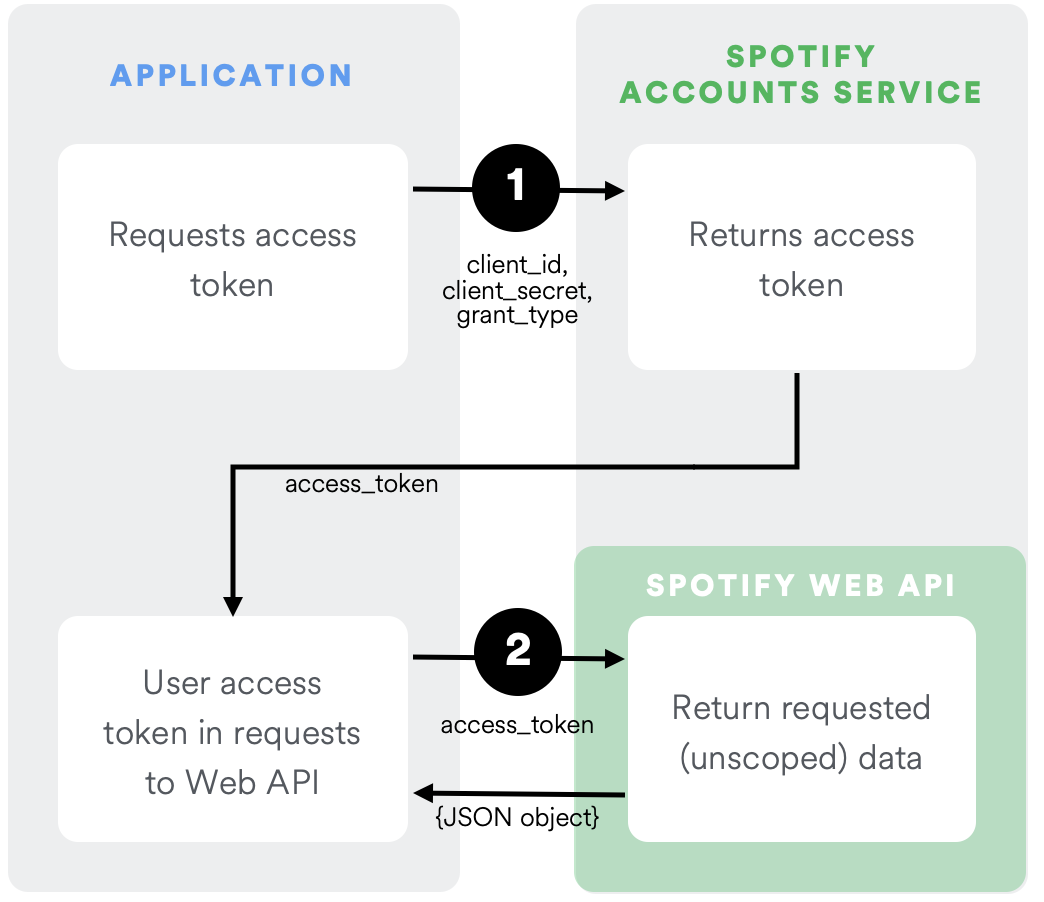
\includegraphics[width=0.6\textwidth]{SpotifyAuthFlow}
    \\
    Source: \cite{SpotifyAuth}
\end{figure}

Step one is a post request to the Spotify Account Service with the client id and client secret from the application dashboard, which returns an
access token, that is valid for one hour. This token can be used to access any endpoint of the actual \ac{API} that
does not require user specific data. When the token expires, a new one has to be requested before querying the \ac{API} again.
Figure \ref{fig:Access Token Request} shows the full request and response to acquire the token.

\begin{figure}[H]
    \caption{Access Token Request}
	\label{fig:Access Token Request}
\end{figure}
\begin{apiRoute}{post}{https://accounts.spotify.com/api/token}{request access token}
    \begin{routeRequest}{application/x-www-form-urlencoded}
        \begin{routeRequestBody}
{
    "grant_type": "client_credentials",
    "client_id": client id from application dashboard,
    "client_secret": client secret from dashboard
}
        \end{routeRequestBody}
    \end{routeRequest}
    \begin{routeResponse}{application/json}
        \begin{routeResponseItem}{200}{ok}
            \begin{routeResponseItemBody}
{
    "access_token": "BQDgQCSx-tIMDo9LfVeZxm6YMl2p_WbEU3Q9ENsVl7e--6d_vockTsfzMVUhPWiHSSnFUuHvm_9POA1kYEw",
    "token_type": "Bearer",
    "expires_in": 3600
}
            \end{routeResponseItemBody}
        \end{routeResponseItem}
    \end{routeResponse}
\end{apiRoute}

In the Python implementation, the requests library is used to execute the request in figure \ref{fig:Access Token Request}
and store the access token in a variable. The dotenv library is used to read the client id and secret from a seperate
.env file, rather than writing it into the code. This prevents these sensitive credentials from being committed
into version control, which is hosted in a public GitHub repository and would therefore make the credentials public.

\begin{lstlisting}[language=Python]
    #Get environment variables from ".env" file and read credentials
    load_dotenv('.env')
    client_id = os.environ.get('CLIENT_ID')
    client_secret = os.environ.get('CLIENT_SECRET')
    
    # Authenticate and get an API Token from Spotify using a Client ID and secret
    def getAuthTokenFromCredentials(id, secret):
    
        url = "https://accounts.spotify.com/api/token"
    
        payload = f'grant_type=client_credentials&client_id={id}&client_secret={secret}'
        headers = {
        'Content-Type': 'application/x-www-form-urlencoded',
        }
    
        response = requests.request("POST", url, headers=headers, data=payload)
    
        return response.json()["access_token"]
    
    auth_token = getAuthTokenFromCredentials(client_id, client_secret)
\end{lstlisting}

\subsubsection{Getting Features}

In order to predict the genre of a track based on audio features, these features have to be requested
for every track. Spotify provides an endpoint to get audio features for a single track or up to 50 tracks at
a time. The latter is used in the Python implementation as it reduces the number of requests to be made.
The typical request/response pattern for the audio-request endpoint of a single track is shown in
figure \ref{fig:Audio Feature Request}.

\begin{figure}[H]
    \caption{Audio Feature Request}
	\label{fig:Audio Feature Request}
\begin{apiRoute}{get}{https://api.spotify.com/v1/audio-features/\{id\}}{request audio features for id}
    \methodJson
    \begin{routeParameter}
        \routeParamItem{id}{id of the song}
    \end{routeParameter}
    \begin{routeResponse}{application/json}
        \begin{routeResponseItem}{200}{ok}
            \begin{routeResponseItemBody}
{
    "danceability": 0.677,
    "energy": 0.638,
    "key": 8,
    "loudness": -8.631,
    "mode": 1,
    "speechiness": 0.333,
    "acousticness": 0.589,
    "instrumentalness": 0,
    "liveness": 0.193,
    "valence": 0.435,
    "tempo": 82.810,
    "type": "audio_features",
    "id": "2e3Ea0o24lReQFR4FA7yXH",
    "uri": "spotify:track:2e3Ea0o24lReQFR4FA7yXH",
    "track_href": "https://api.spotify.com/v1/tracks/2e3Ea0o24lReQFR4FA7yXH",
    "analysis_url": "https://api.spotify.com/v1/audio-analysis/2e3Ea0o24lReQFR4FA7yXH",
    "duration_ms": 211497,
    "time_signature": 4
}
            \end{routeResponseItemBody}
        \end{routeResponseItem}
    \end{routeResponse}
\end{apiRoute}
\end{figure}

With the exception of type, id, uri, track\_href and analysis\_url, all of the fields included in this response
can be used as features in the dataset. However, this api call expects a track id, which we need to get using
other api calls first. This could be a search endpoint, getting all tracks in a playlist, etc.
Also, it does not give the track or artist names and doesn't include a genre.

\subsubsection{Getting Track IDs and Labels}

There is no simple endpoint that takes one or more track ids and returns  a "genre" field
in its response. The exploration of the API using the reference, web console and Postman only revealed
two ways of getting the genre of a track. 

The first way is using the artist of a track. Given a track id, the artists of the track and their corresponding
ids can be requested by using the "/tracks/{id}" endpoint. Then, using the artist id, the genres that an
artist is known for are returned, as can be seen in figure \ref{fig:Artist Request}.

\begin{figure}[H]
    \caption{Artist Request}
	\label{fig:Artist Request}
\begin{apiRoute}{get}{https://api.spotify.com/v1/artists/\{id\}}{request information about an artist by their id}
    \begin{routeParameter}
        \routeParamItem{id}{id of the artist}
    \end{routeParameter}
    \begin{routeResponse}{application/json}
        \begin{routeResponseItem}{200}{ok}
            \begin{routeResponseItemBody}
{
    "external_urls": {
        "spotify": "https://open.spotify.com/artist/6l3HvQ5sa6mXTsMTB19rO5"
    },
    "followers": {
        "href": null,
        "total": 15554811
    },
    "genres": [
        "conscious hip hop",
        "hip hop",
        "north carolina hip hop",
        "rap"
    ],
    "href": "https://api.spotify.com/v1/artists/6l3HvQ5sa6mXTsMTB19rO5",
    "id": "6l3HvQ5sa6mXTsMTB19rO5",
    "images": [
        ...
    ],
    "name": "J. Cole",
    "popularity": 89,
    "type": "artist",
    "uri": "spotify:artist:6l3HvQ5sa6mXTsMTB19rO5"
    }
            \end{routeResponseItemBody}
        \end{routeResponseItem}
    \end{routeResponse}
\end{apiRoute}
\end{figure}

This examplary API response shows a problem with this approach. One artist can be sorted
into multiple genres.
A given track might be associated with either of the artists genres, but the data does
not show, which one exactly.
Additionally a track might have multiple artists which further complicates this.
Given these circumstances, this approach is problematic.

The second way is Spotifys "categories" feature. The apps search tab provides a number of
categories that a user can browse through to find new music in their preferred genre or style.
In figure \ref{fig:Categories and Playlists in Spotify App}a an overview over some of the categories
that are available in the Spotify App is shown. There are categories of multiple types, e.g.
specific activities, like Cooking or Gaming, or places, like "At Home" or "In the Car".
But there are also categories for nearly all major genres. In the app screenshot
there is for example Classical, Jazz or Soul.
These categories can be used to get tracks that belong in each specific category. When a user taps on
a one of the categories, playlists that contain tracks of the respective category are shown to the user,
like shown in figure \ref{fig:Categories and Playlists in Spotify App}b.
The API mirrors the apps behaviour and provides an endpoint to get a list of categories and their ids,
one to get all playlists and playlist\_ids in a category, and one to get all tracks and track\_ids in
a playlist. This chain of API calls is used to request every track in every playlist in a certain category.

\begin{figure}[H]
    \centering
    \subfloat[\centering Category Overview]{{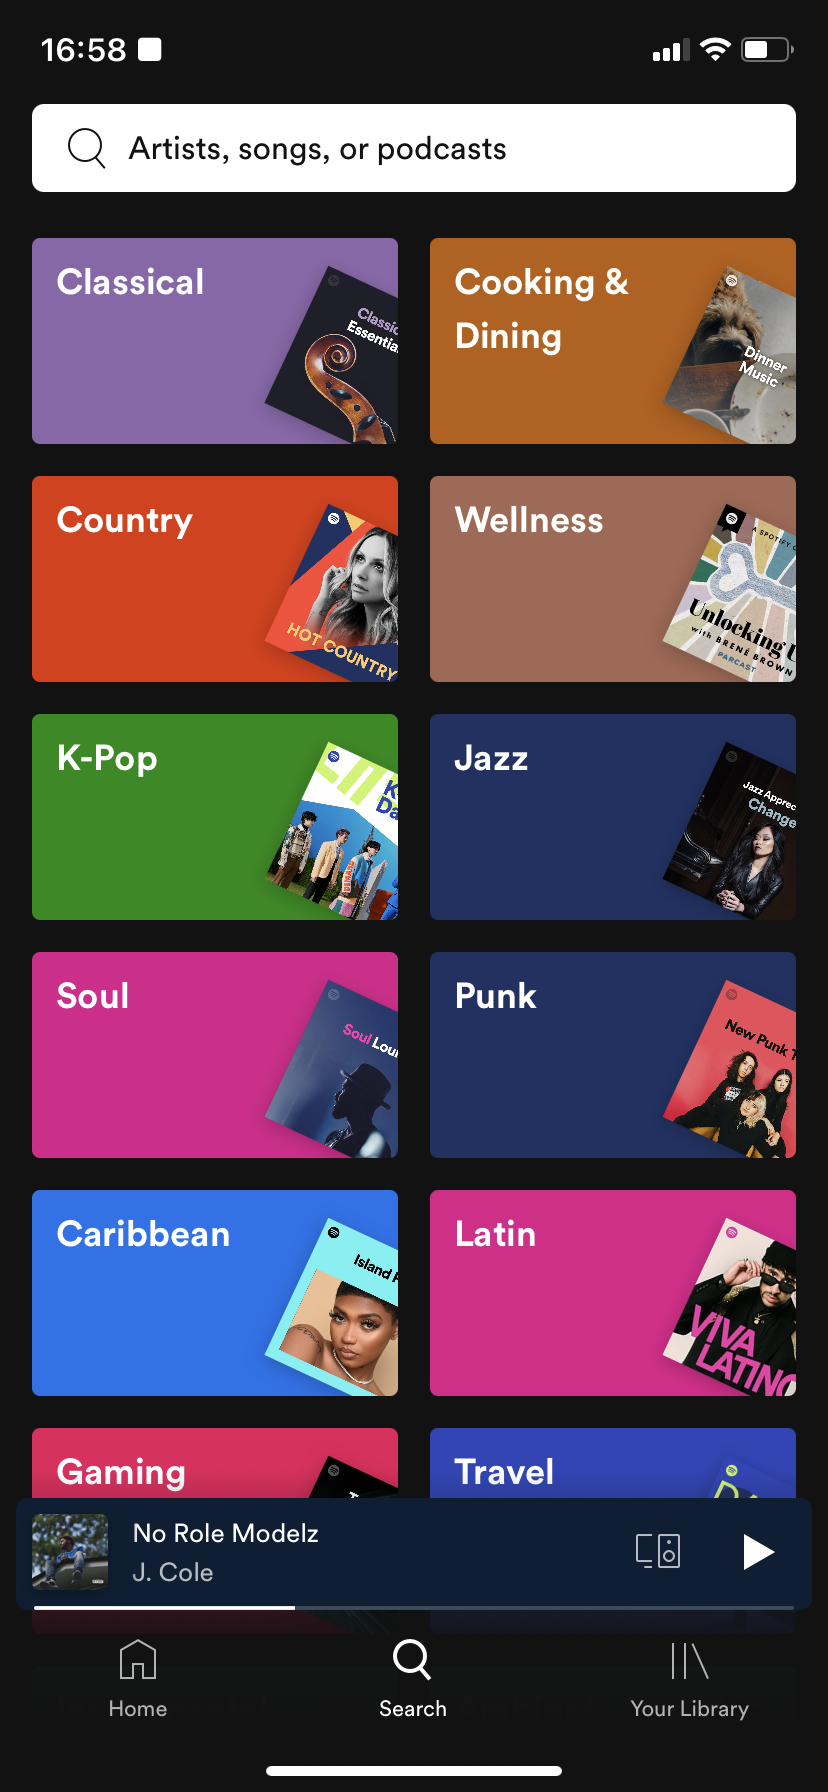
\includegraphics[width=4cm]{SpotifyCategoryOverview} }}%
    \qquad
    \subfloat[\centering Playlists in category]{{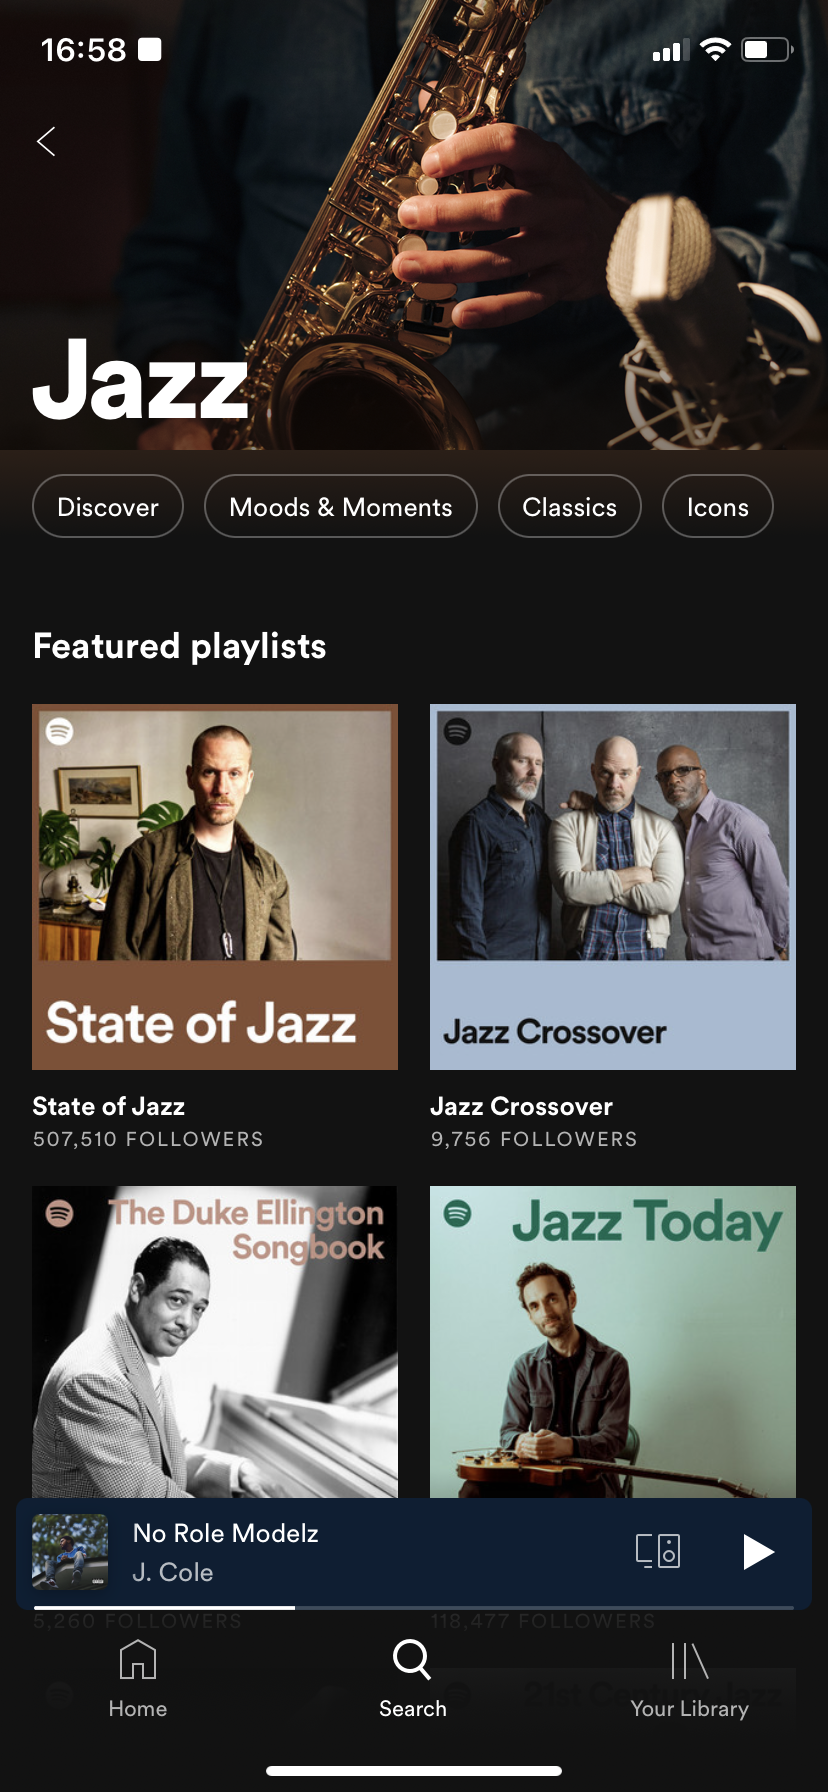
\includegraphics[width=4cm]{SpotifyPlaylistOverview} }}%
    \caption{Categories and Playlists in Spotify App}%
    \label{fig:Categories and Playlists in Spotify App}%
\end{figure}

